\documentclass{article}
\usepackage{graphicx} % Required for inserting images
\usepackage{amsmath}
\usepackage{geometry}
\usepackage{amssymb}
\usepackage{color}
\usepackage{CJKutf8}
\usepackage{float}
\usepackage{subfigure}
\usepackage{listings}
\usepackage{placeins}
\usepackage{enumitem}
\geometry{a4paper, scale=0.8}   
\linespread{2}
\definecolor{dark_green}{RGB}{0,102,51}
\title{Lab2 - UDP}
\author{Jiaxi Zhang}
\date{\today}
\begin{document}
\maketitle
\begin{CJK*}{UTF8}{gbsn}

\section{How many fields there are in the UDP header}
Four fields: Source Port, Destination Port, Length, Checksum.
\begin{figure}[H]
    \centering
    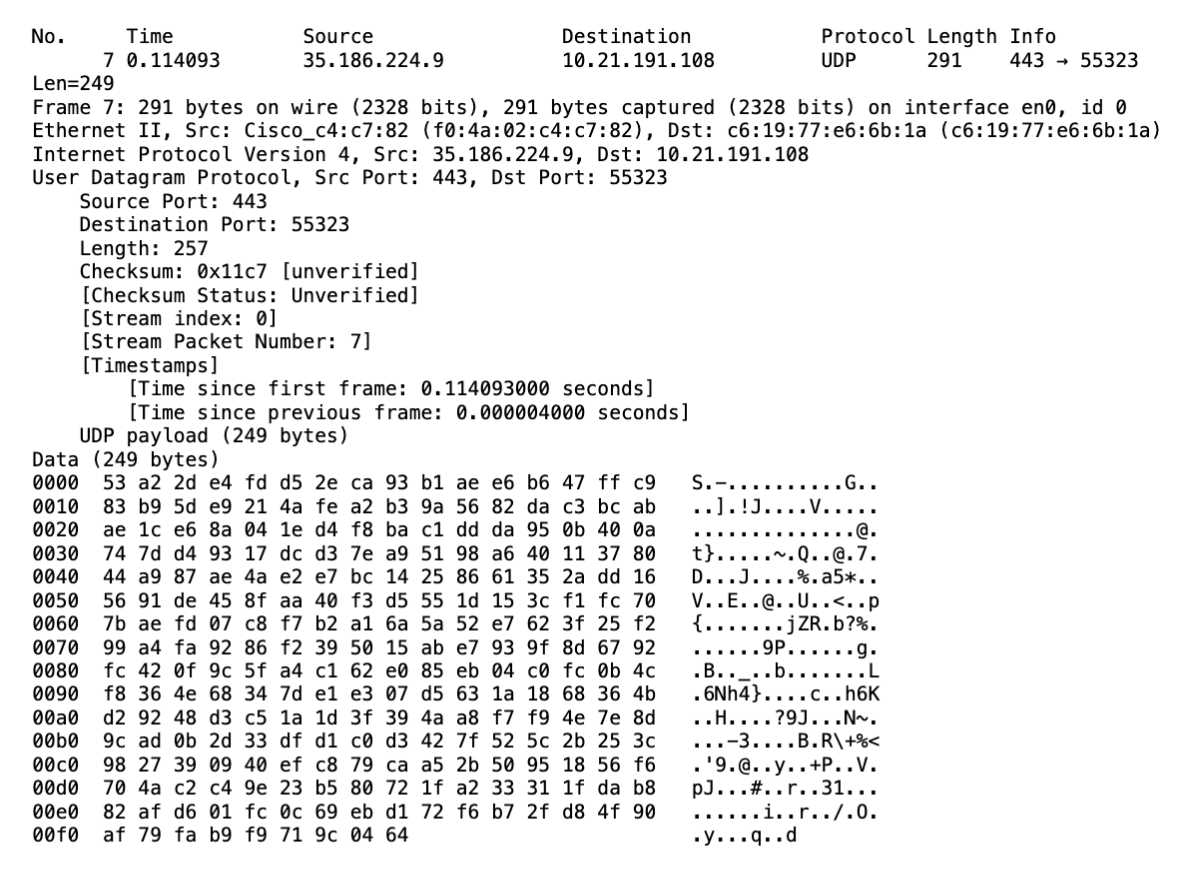
\includegraphics[width=0.8\textwidth]{Q1 - PrintOut.png}
    \caption{PrintOut for Question 1}
\end{figure}

\section{The Length of each field in the UDP header}
\begin{itemize}
    \item Source Port: 2 bytes
    \item Destination Port: 2 bytes
    \item Length: 2 bytes
    \item Checksum: 2 bytes
\end{itemize}
8 bytes in total.
It can be seen in the screenshot below since the length is highlighted in the packet details.
\begin{figure}[H]
    \centering
    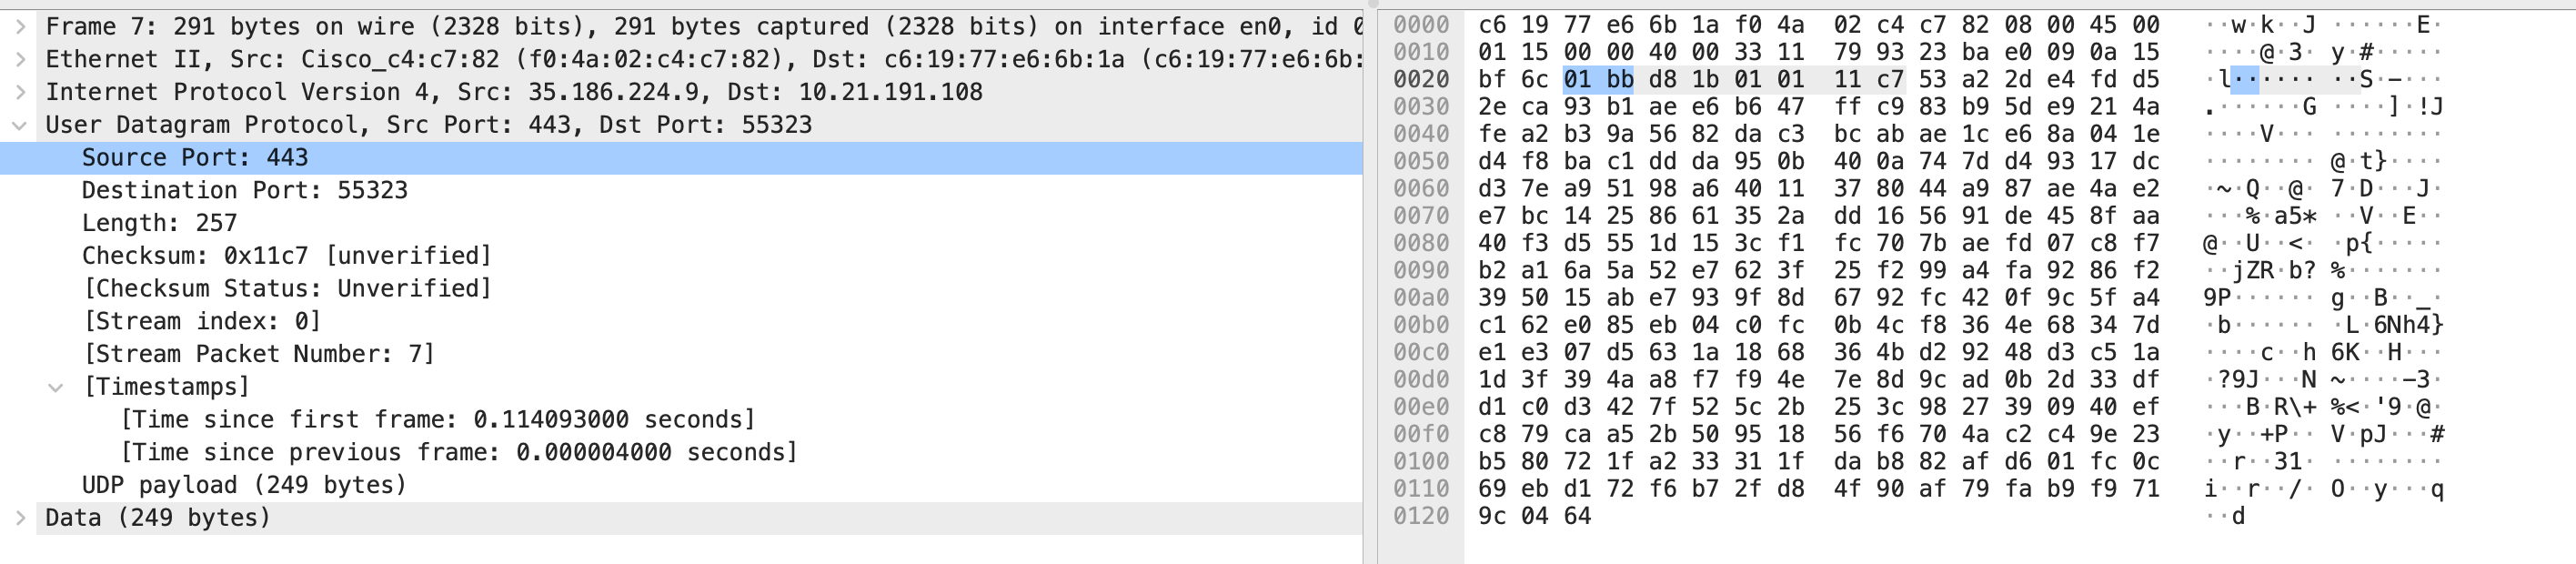
\includegraphics[width=0.8\textwidth]{Q2 - PrintOut1.png}
\end{figure}
\begin{figure}[H]
    \centering
    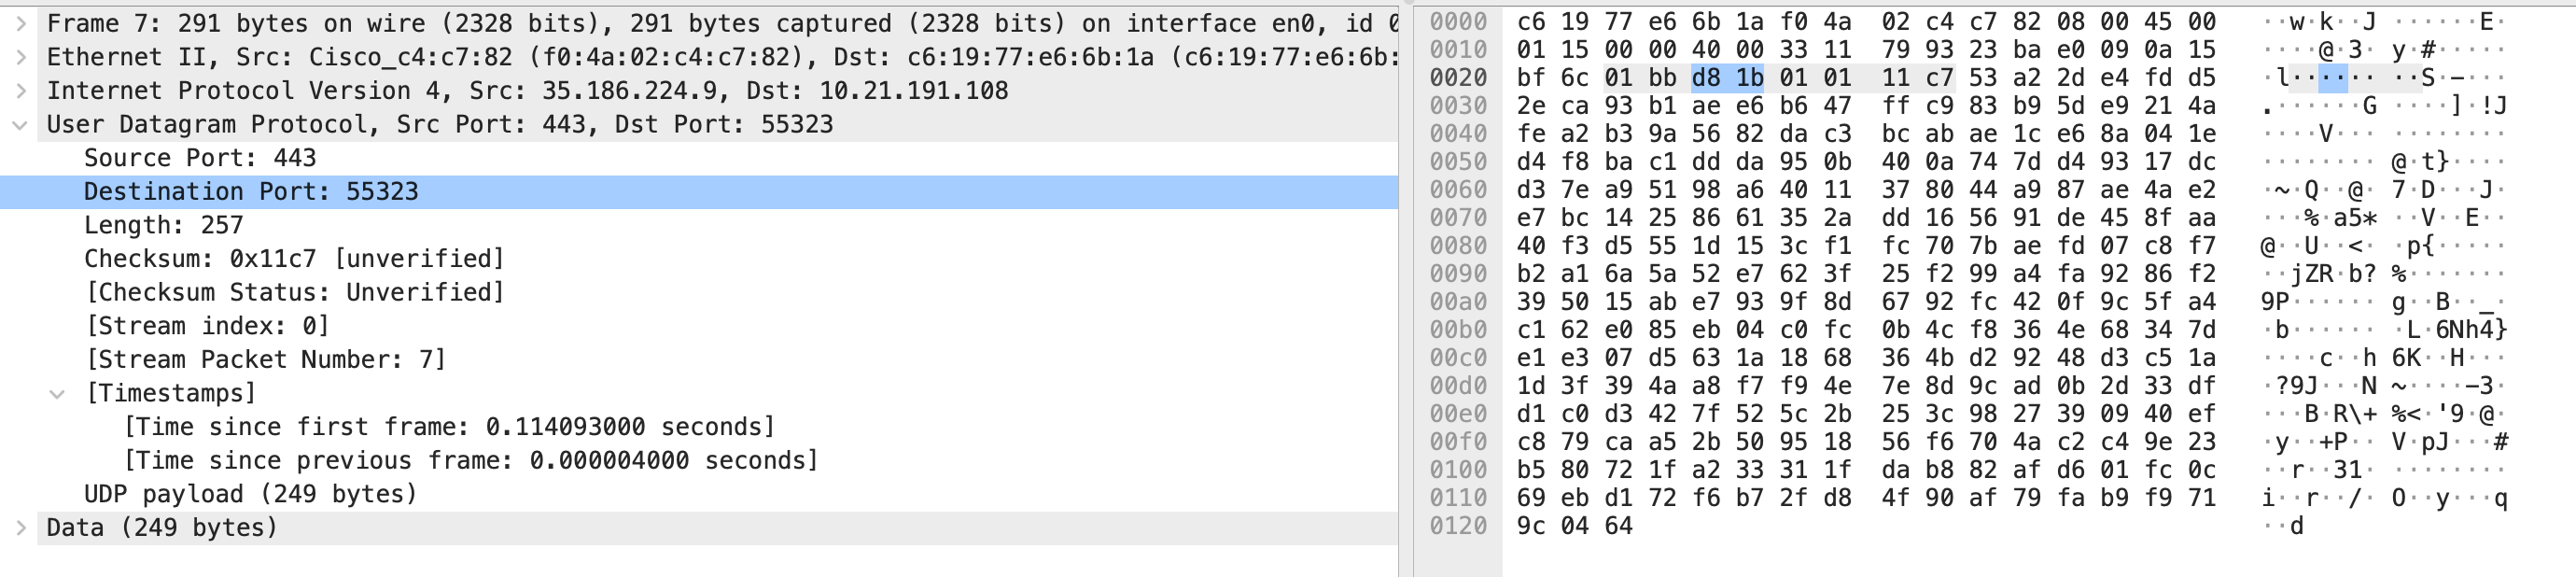
\includegraphics[width=0.8\textwidth]{Q2 - PrintOut2.png}
\end{figure}
\begin{figure}[H]
    \centering
    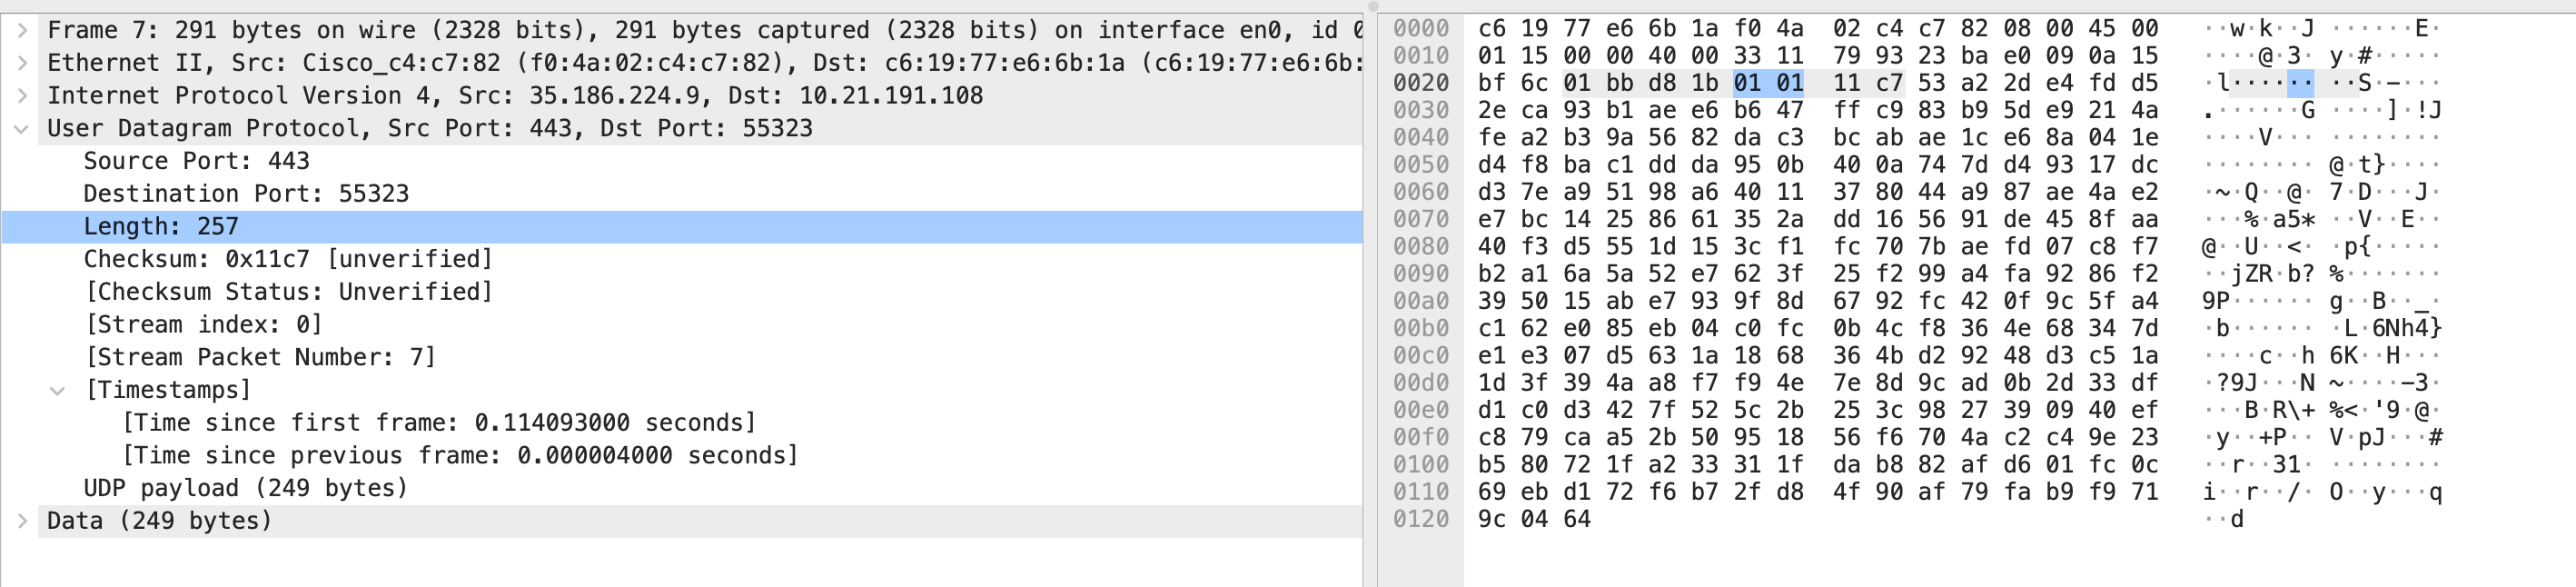
\includegraphics[width=0.8\textwidth]{Q2 - PrintOut3.png}
\end{figure}
\begin{figure}[H]
    \centering
    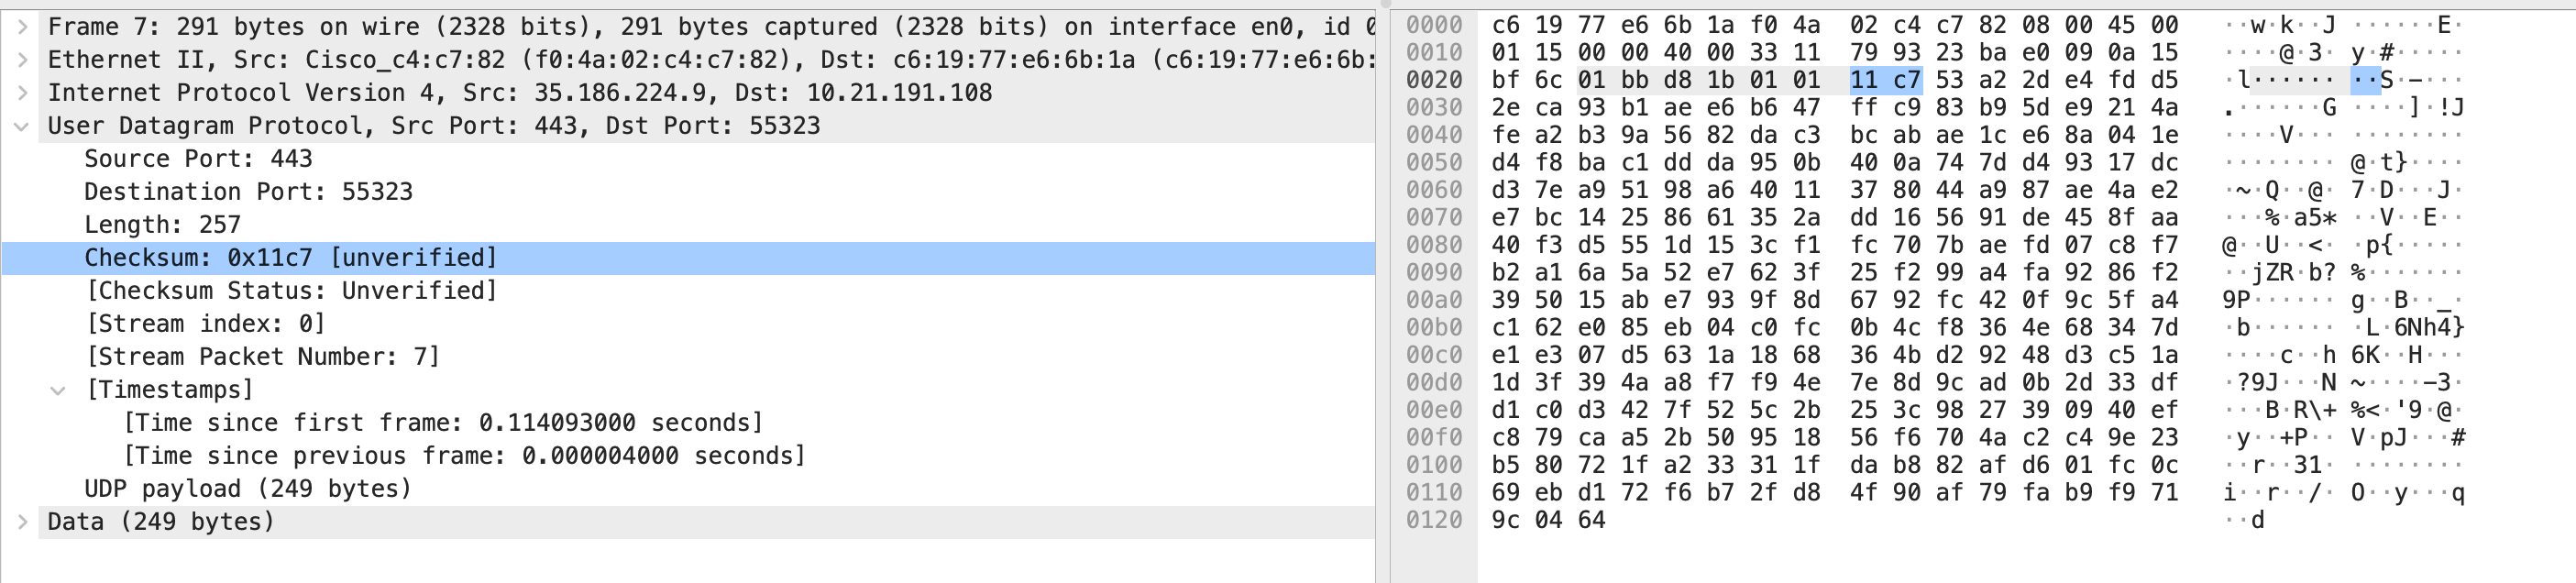
\includegraphics[width=0.8\textwidth]{Q2 - PrintOut4.png}
\end{figure}
\end{CJK*}

\section{Length Field}
The value of the Length field indicates the length of the UDP header and the data(payload) in bytes.
The header length is 8 (2*4) bytes, and the data is 249 bytes. Therefore, the total length is 257 bytes.
It can be seen in the screenshot below.
\begin{figure}[H]
    \centering
    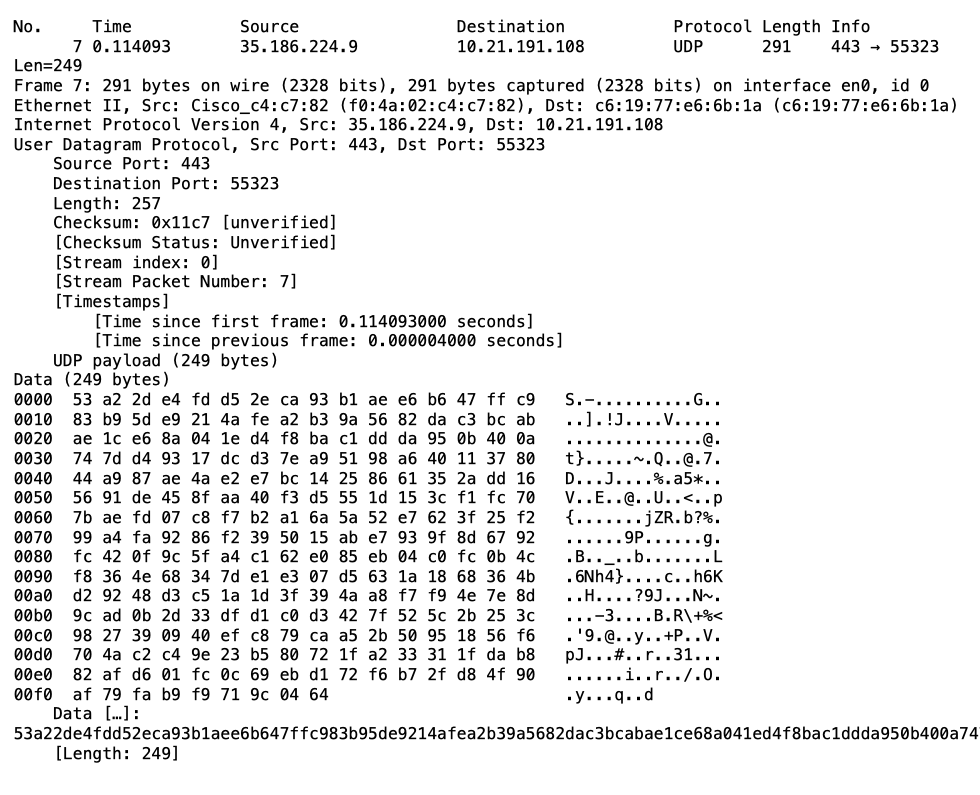
\includegraphics[width=0.8\textwidth]{Q3 - PrintOut.png}
    \caption{PrintOut for Question 3}
\end{figure}

\section{Max Length of the UDP Payload}
The maximum length of the UDP payload is 65527 bytes. In the second question,
we knew that the length field is 2 bytes, which means the maximum value is $2^{16} - 1 = 65535$.
And the 8 bytes of the header should always be included. Therefore, the maximum length of the UDP payload is 65527 bytes.

\section{Largest possible source port number}
The largest possible source port number is $2^{16} - 1 = 65535$.

\section{Protocol number for UDP}
The protocol number for UDP is 17 and 0x11 in hexadecimal.
\begin{figure}[H]
    \centering
    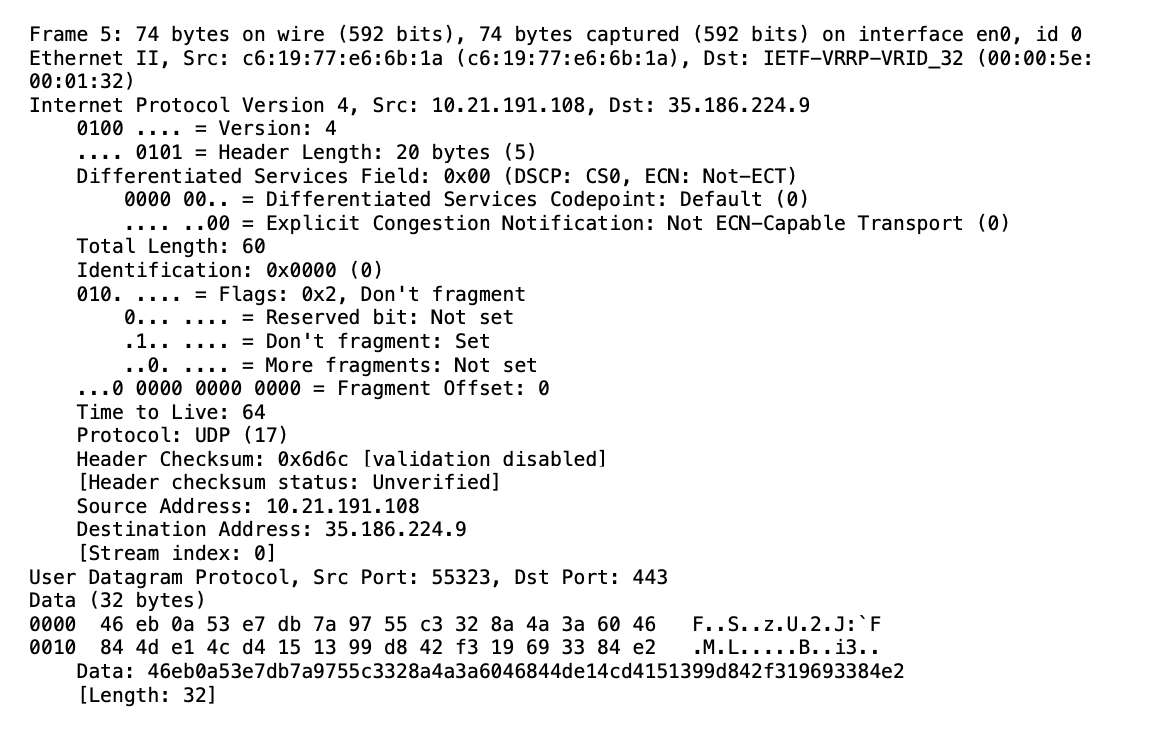
\includegraphics[width=0.8\textwidth]{Q6 - PrintOut.png}
    \caption{PrintOut for Question 6}
\end{figure}
\section{Pair Packets}
The Source Port and Destination Port of the two packets are exchanged.
In the first packet, the Source Port is 55323 and the Destination Port is 443,
while in the second packet, the Source Port is 443 and the Destination Port is 55323.
The two hosts are using the same ports to communicate with each other.
\begin{figure}[H]
    \centering
    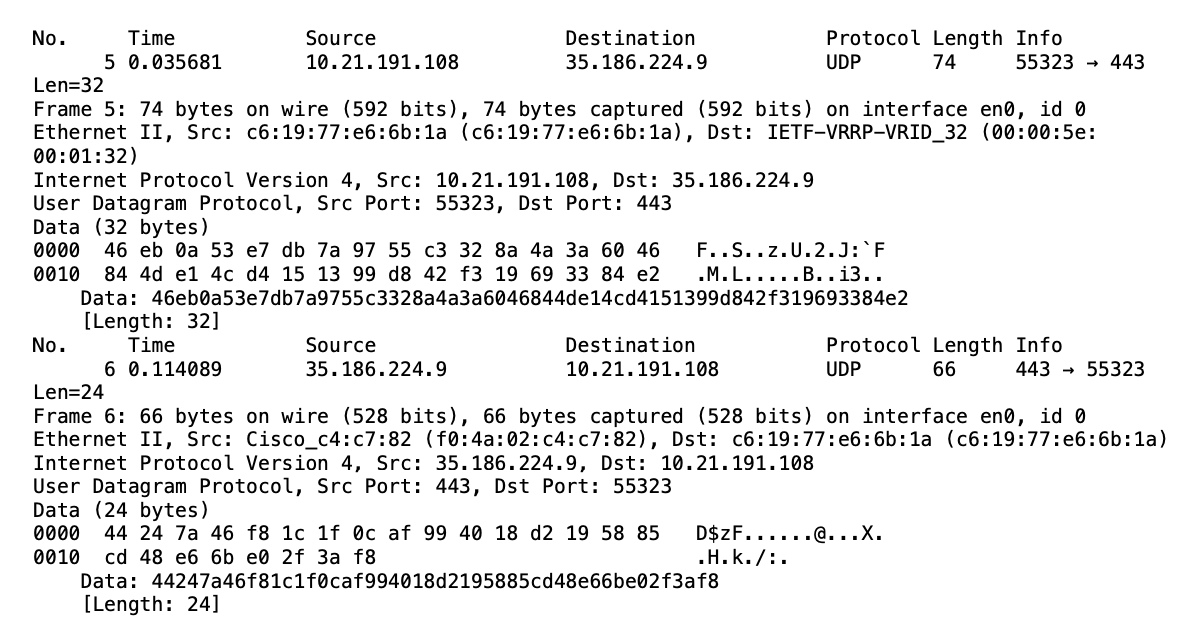
\includegraphics[width=0.8\textwidth]{Q7 - PrintOut.png}
    \caption{PrintOut for Question 7}
\end{figure}
\end{document}
